\PassOptionsToPackage{dvipsnames}{xcolor}
\documentclass{cubeamer}

\usepackage{xcolor}
\usepackage{multimedia}
\usepackage{caption}
\usepackage{subcaption}
\usepackage{bigintcalc}


\title{Soutenance Stage G1}
\subtitle{Intelligence Artificiel et Santé}
\author[Nicolás Acevedo]{Stagiaire : Nicolás Acevedo \\ Tuteur : Hayfa Zgaya}
\date{17 février 2021} % or whatever the date you are presenting in is
\institute[École Centrale de Lille]{}
%\copyrightnotice{Published by the American Institute of Aeronautics and Astronautics, Inc., with permission}

\newcommand{\tab}{\- \- \- \-}
\begin{document}
	
\maketitle

%\cutoc

\section{Introduction}

\begin{frame}
	\begin{figure}
		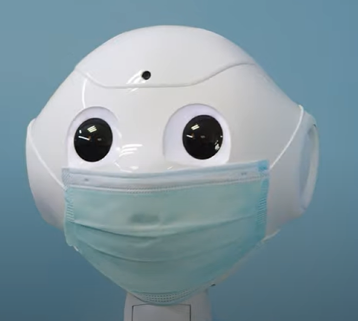
\includegraphics[height = 0.7\textheight]{img/peppermask.png}
	\end{figure}
\end{frame}

\begin{frame}
\begin{minipage}{.49\textwidth}
\begin{figure}
	\begin{subfigure}{.45\textwidth}
		\centering
		% include first image
		
\includegraphics[width=.8\linewidth]{img/pm1.jpg}  
	\end{subfigure}
	\begin{subfigure}{.45\textwidth}
		\centering
		% include second image
		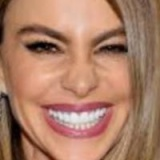
\includegraphics[width=.8\linewidth]{img/pm2.jpg}  
	\end{subfigure}

	\begin{subfigure}{.45\textwidth}
		\centering
		% include third image
		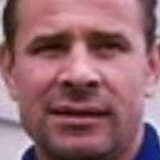
\includegraphics[width=.8\linewidth]{img/pm3.jpg}  
	\end{subfigure}
	\begin{subfigure}{.45\textwidth}
		\centering
		% include fourth image
		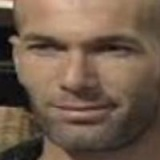
\includegraphics[width=.8\linewidth]{img/pm4.jpg}  
	\end{subfigure}
	\caption{Pas de Masque}
\end{figure}
\end{minipage}
\begin{minipage}{.49\textwidth}
	
\begin{figure}
	\begin{subfigure}{.45\textwidth}
		\centering
		% include first image
		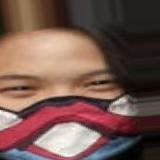
\includegraphics[width=.8\linewidth]{img/am1.jpg}  
	\end{subfigure}
	\begin{subfigure}{.45\textwidth}
		\centering
		% include second image
		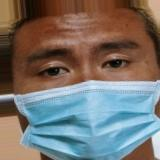
\includegraphics[width=.8\linewidth]{img/am2.jpg}  
	\end{subfigure}
	
	\begin{subfigure}{.45\textwidth}
		\centering
		% include third image
		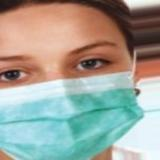
\includegraphics[width=.8\linewidth]{img/am3.jpg}  
	\end{subfigure}
	\begin{subfigure}{.45\textwidth}
		\centering
		% include fourth image
		
\includegraphics[width=.8\linewidth]{img/am4.jpg}  
	\end{subfigure}
	\caption{Avec Masque}
\end{figure}
\end{minipage}

\end{frame}

\section{Implementation}

\begin{frame}[fragile]
\begin{semiverbatim}
import cv2
import os
import numpy as np
import tensorflow as tf
import qi
import sys

prototxt_path = os.path.join('resources/deploy.prototxt')
caffemodel_path = os.path.join('resources/weights.caffemodel')
model = cv2.dnn.readNetFromCaffe(prototxt_path, caffemodel_path)

modelMasque = tf.keras.models.load_model("QSTOMIT-MASQUE.model")
	\end{semiverbatim}
	
\end{frame}

\begin{frame}[fragile]
\begin{semiverbatim}
session = qi.Session()
session.connect("tcp://192.168.0.102:9559")

tts = session.service("ALTextToSpeech")

camera = session.service("ALVideoDevice")
camera_top = camera.subscribeCamera("camera_top", 0, 2, 11, 30)
\end{semiverbatim}
\end{frame}

\begin{frame}[fragile]
\begin{semiverbatim}
while True:

\tab image = camera.getImageRemote(camera_top)
\tab h = image[0]
\tab w = image[1]
\tab image = np.array(image[6])
\tab image = np.reshape(image, (w, h, 3))
\tab image = cv2.cvtColor(image, cv2.COLOR_BGR2RGB)
\tab blob = cv2.dnn.blobFromImage(cv2.resize(image, (300, 300)), 1.0, 
\tab \tab \tab (300, 300), (104.0, 177.0, 123.0))
\tab model.setInput(blob)
\tab detections = model.forward()
\end{semiverbatim}
\end{frame}

\begin{frame}[fragile]
\begin{semiverbatim}
for i in range(0, detections.shape[2]):
\tab box = detections[0, 0, i, 3:7] * np.array([w, h, w, h])
\tab (startX, startY, endX, endY) = box.astype("int")

\tab confidence = detections[0, 0, i, 2]

\tab if (confidence > 0.5):
\tab \tab frame = image[startY:endY, startX:endX]

\tab \tab capture = cv2.resize(frame, (224, 224))
\tab \tab capture = capture.reshape((1, capture.shape[0], capture.shape[1],\ \tab \tab \tab \tab \tab capture.shape[2]))
\tab \tab predict = modelMasque.predict(capture)
\end{semiverbatim}
\end{frame}

\begin{frame}[fragile]
\begin{semiverbatim}
pasDeMasque = predict[0][0]
avecMasque = predict[0][1]

pM_counter = aM_counter = 0

if pasDeMasque > avecMasque:
\tab pM_counter += 1
else:
\tab aM_counter += 1
\end{semiverbatim}
\end{frame}

\begin{frame}[fragile]
\begin{semiverbatim}
if pM_counter > 1:
\tab tts.say("Il y a "+str(pM_counter)+" personnes sans masque, mettre votre masque s'il vous plaît")
elif pM_counter == 1:
\tab tts.say("Vous ne porte pas votre masque, mettre votre masque s'il vous plaît")
elif pM_counter == 0 and aM_counter > 0:
\tab tts.say("Merci d'utiliser votre masque") 
\end{semiverbatim}	
\end{frame}

\section{Résultats}
\begin{frame}
	\begin{columns}
		\column{0.5\textwidth}
		\begin{figure}[H]
			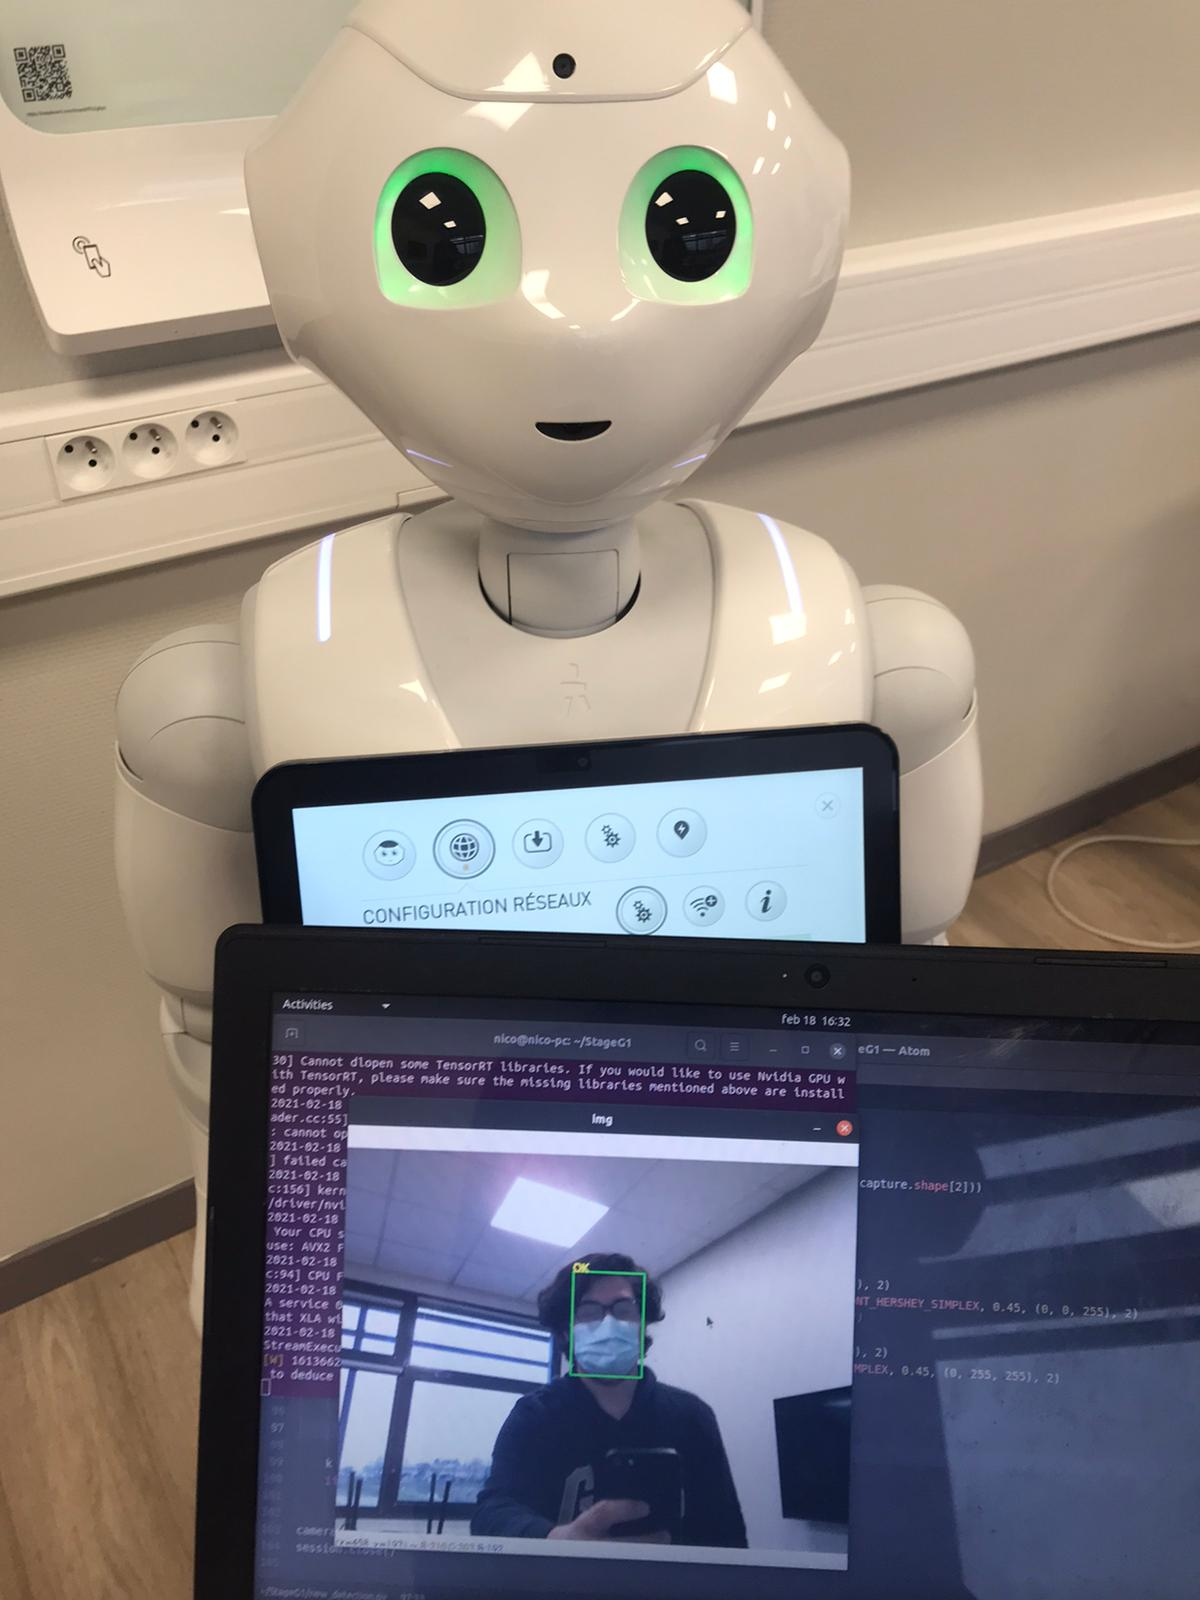
\includegraphics[width = 0.7\textwidth]{img/avecMasque.jpeg}
			\caption{Reconnaissance du porte de masque}
		\end{figure}
		\column{0.5\textwidth}
		\begin{figure}[H]
			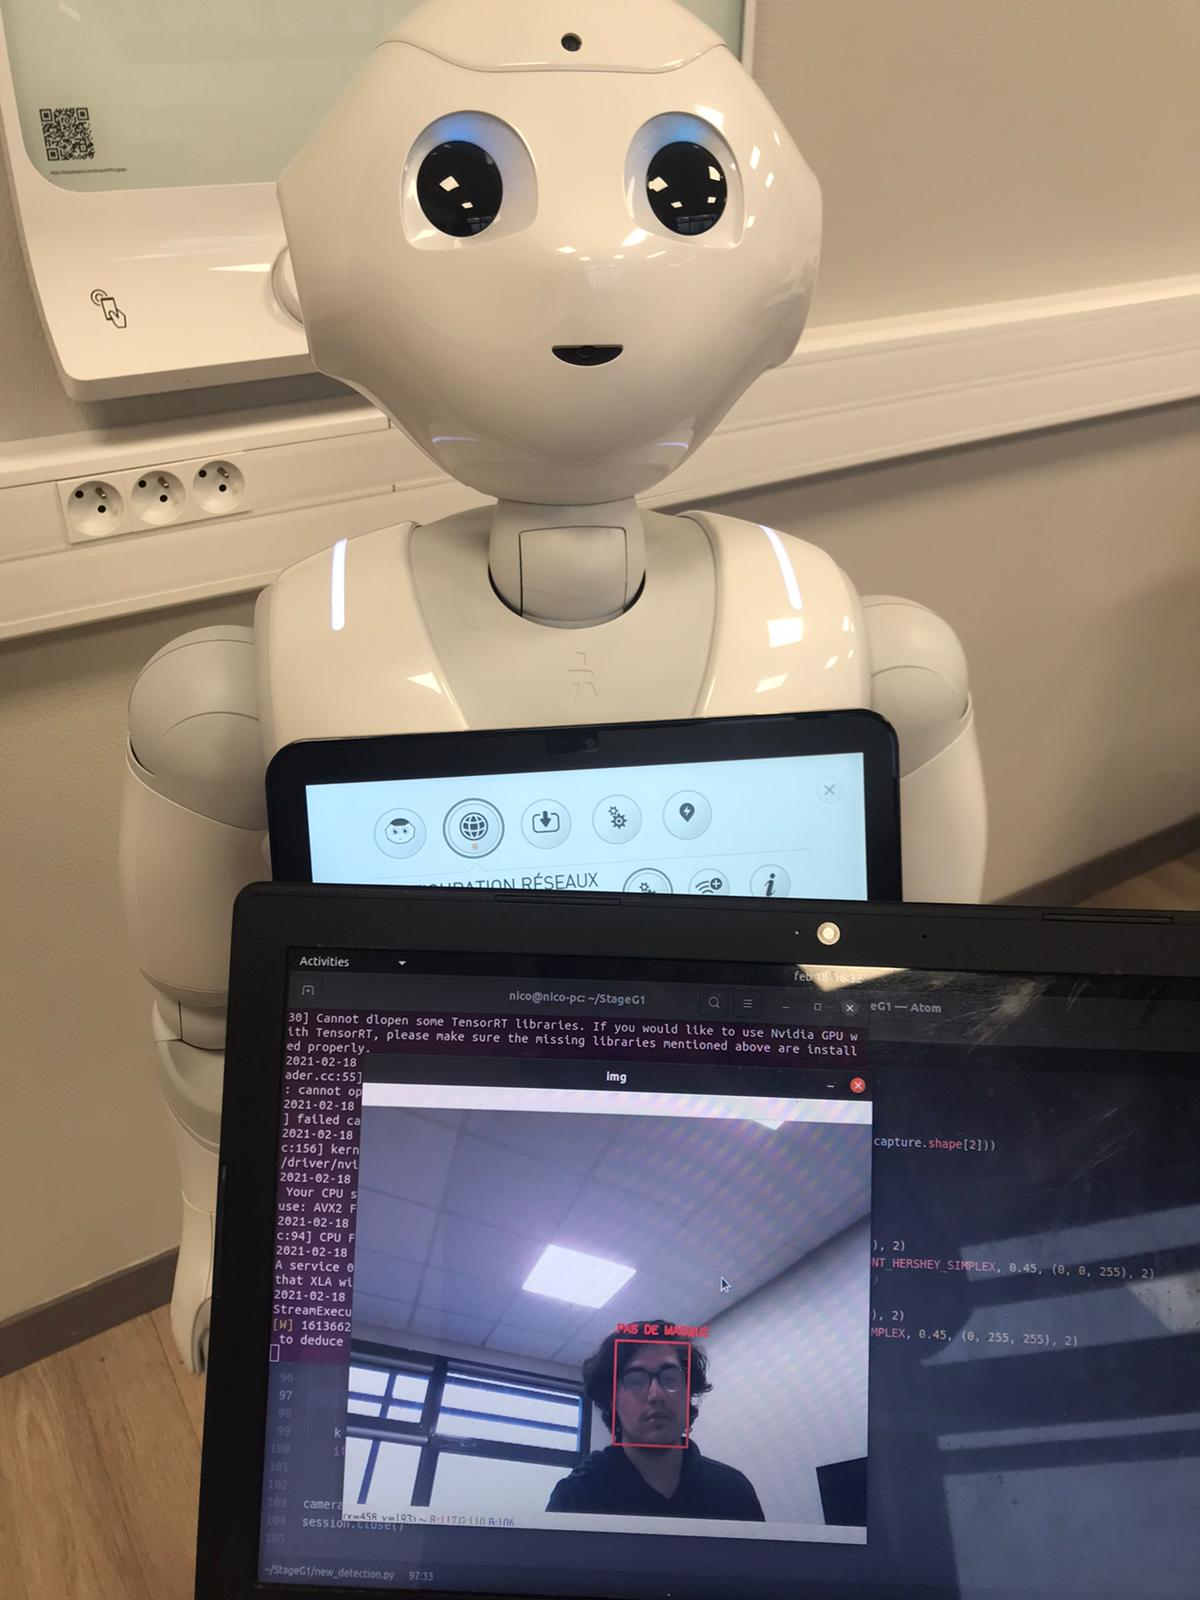
\includegraphics[width = 0.7\textwidth]{img/pasDeMasque.jpeg}
			\caption{Reconnaissance du non-masque}
		\end{figure}
	\end{columns}
\end{frame}

\begin{frame}
	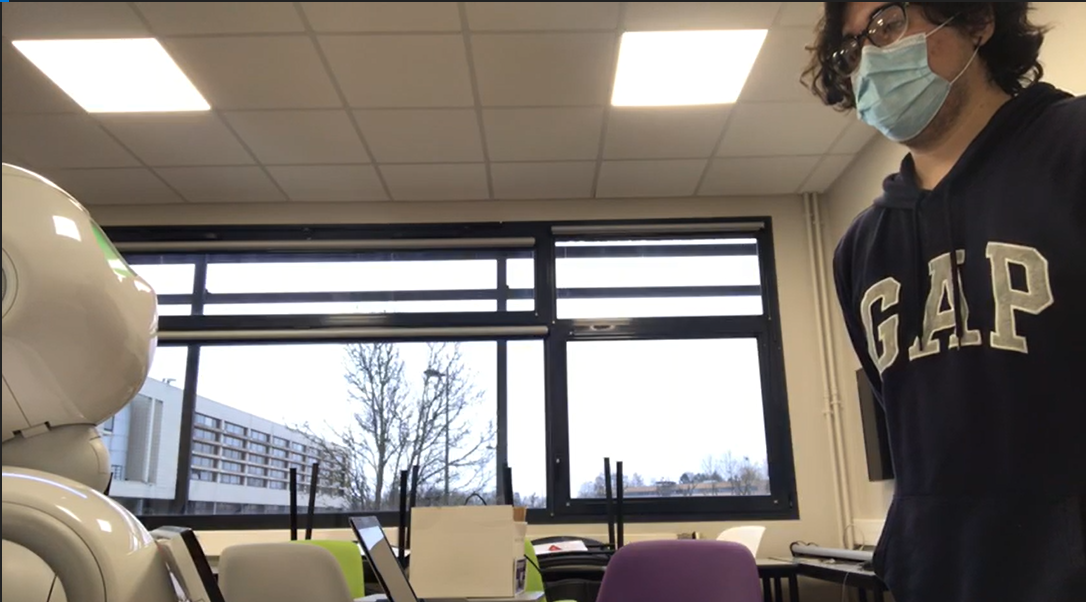
\includegraphics[width = \textwidth]{img/portada.png}
\end{frame}

\end{document}
